% !TeX root = ../main.tex
%
\chapter{Results}\label{chap:results}
The swing-up controller, LQR and the Kalman filter for the twin pendulum are implemented on the system and the the results presented here.
%
%------Swing-Up----------
%
The swing-up controller approaches equilibrium for both pendulums, see \autoref{fig:thetaSwing}. However, when tuning the gain of one pendulum the behavior of the other pendulum is affected.
%
\begin{figure}[H]
  \hspace{-10pt}
  \captionbox
  {
    Swing-up controller attempting to approach equilibrium for both pendulums.
    \label{fig:thetaSwing}
  }
  {
    \hspace{-1cm}
    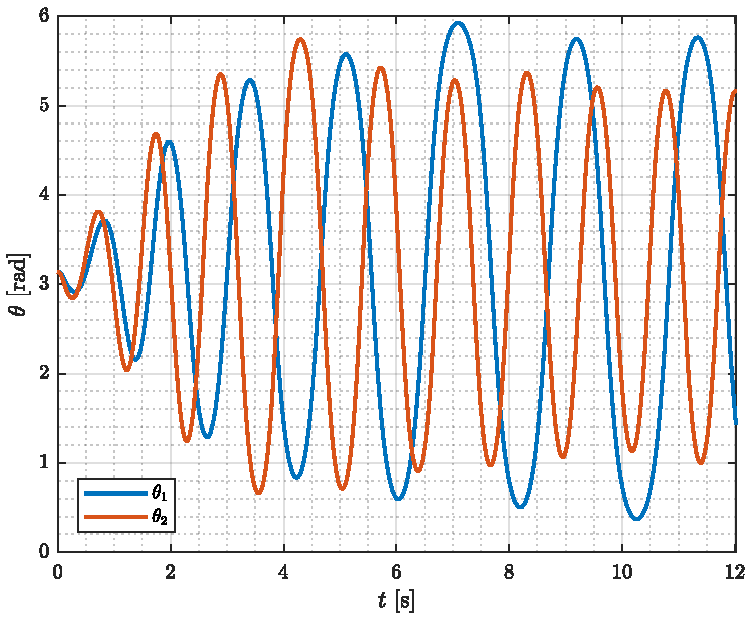
\includegraphics[width=.478\textwidth]{figures/thetaSwing}
  }
  \hspace{20pt}
  \captionbox 
  {
    The position controller keeps the cart within the operating range.
    \label{fig:xSwing}
  }
  {
    \hspace{-1cm}
    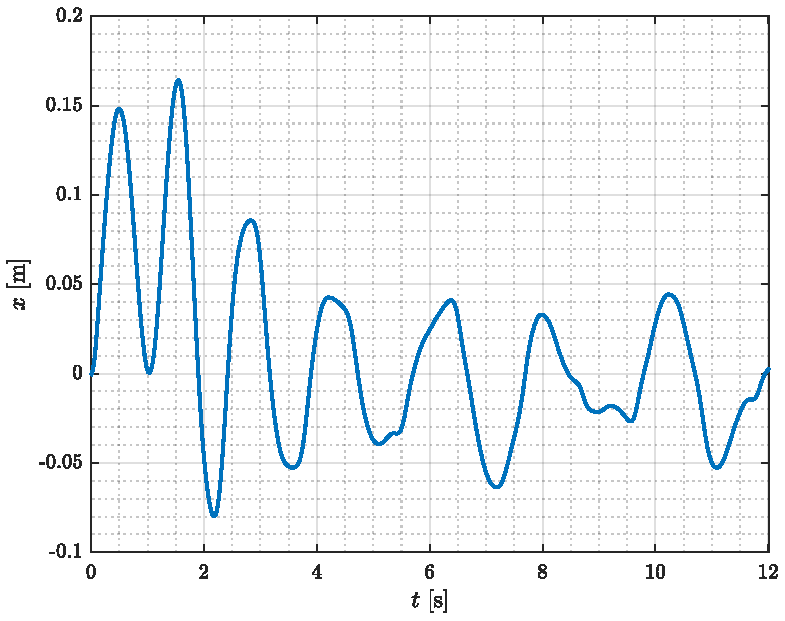
\includegraphics[width=.5\textwidth]{figures/xSwing}
  }  
\end{figure}
%
%
\begin{figure}[H]
  \hspace{-10pt}
  \captionbox
  {
    The energy error of each pendulum. As the first pendulum catches up the second pendulum looses energy.
    \label{fig:EdeltaSwing}
  }
  {
    \hspace{-1cm}
    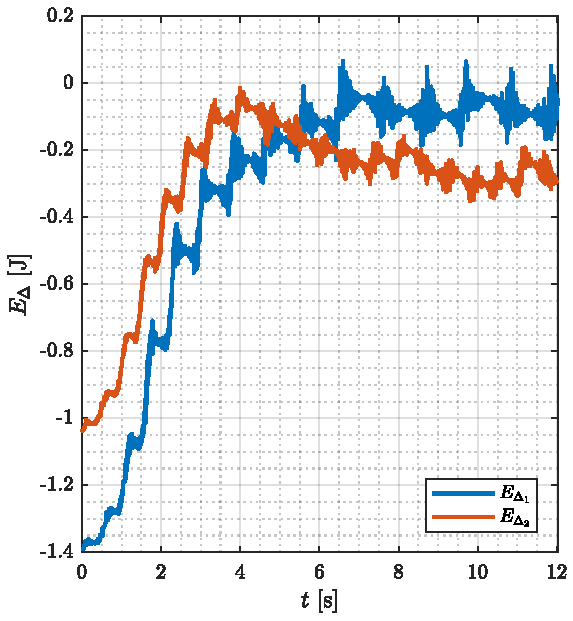
\includegraphics[width=.452\textwidth]{figures/EdeltaSwing}
  }
  \hspace{20pt}
  \captionbox 
  {
    The phase portrait is not symmetrical consistently hitting high velocity after passing $\pi$, downward position.
    \label{fig:phaseSwing}
  }
  {
    \hspace{-1cm}
    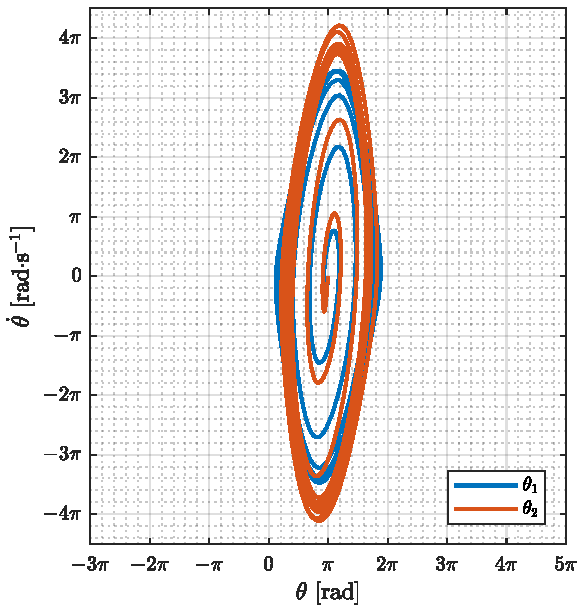
\includegraphics[width=.46\textwidth]{figures/phaseSwing}
  }  
\end{figure}
%The current 
%\begin{figure}[H]
%  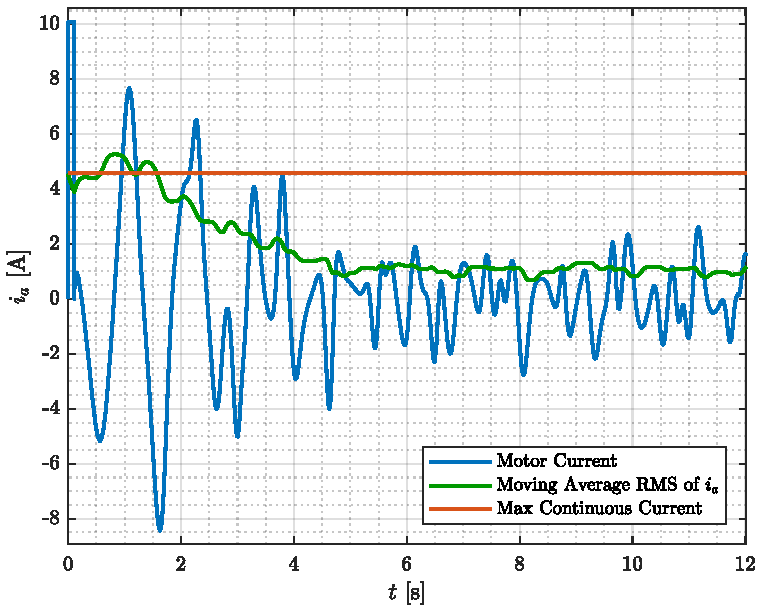
\includegraphics[width=.5\textwidth]{figures/iaSwing}
%  \caption{iaSwing}
%  \label{fig:iaSwing}
%\end{figure}
%
%other available plots
% thetaDotSwing
% xDotSwing
%
This makes it difficult to find the right balance to let both pendulums reach equilibrium at the same time. It is only made more difficult by the position control further adding disturbance to the swing-up controller. \autoref{fig:xSwing} shows the position controller successfully keeping the cart in away from the edges of the rail. In \autoref{fig:EdeltaSwing} the second pendulum first reaches for zero energy error reference, however, as the energy of the first pendulum increases, the second pendulum looses energy. As known from simulations in the design, with more time it should be possible to tune the gains against each other until a balance is achieved and both pendulums approach zero energy error. In \autoref{fig:phaseSwing} the phase portrait is slightly skewed compared to simulation, showing peak velocity after passing $\pi$, the reason is unknown.

%
%------Catch----------
%
A test of the implemented LQR is seen in \autoref{fig:thetaCatch} where both pendulums are started in zero. The controller does keep both pendulums around zero, however with a lot of oscillations.
%
\begin{figure}[H]
  \hspace{-10pt}
  \captionbox
  {
    The LQR successfully keeps both pendulums in upright position.
    \label{fig:thetaCatch}
  }
  {
    \hspace{-1cm}
    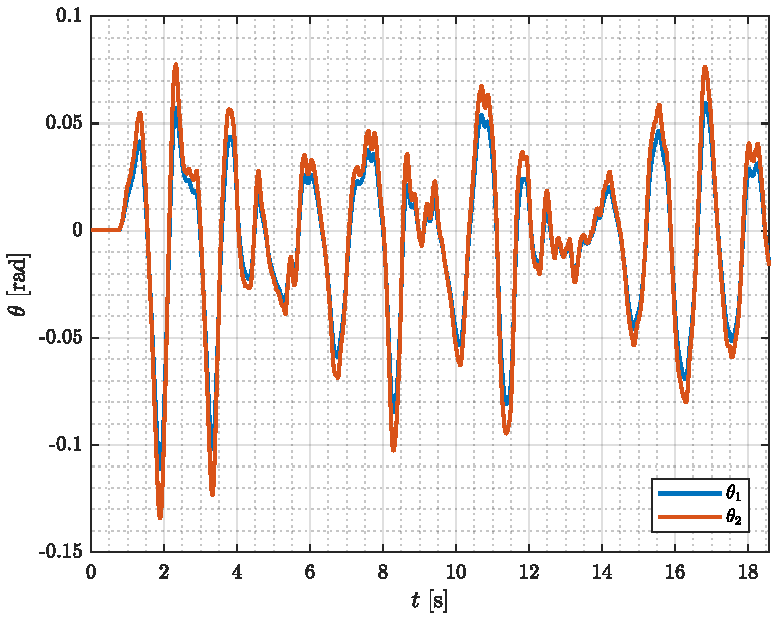
\includegraphics[width=.5\textwidth]{figures/thetaCatch}
  }
  \hspace{20pt}
  \captionbox 
  {
    In this test the cart position is kept close to center.
    \label{fig:xCatch}
  }
  {
    \hspace{-1cm}
    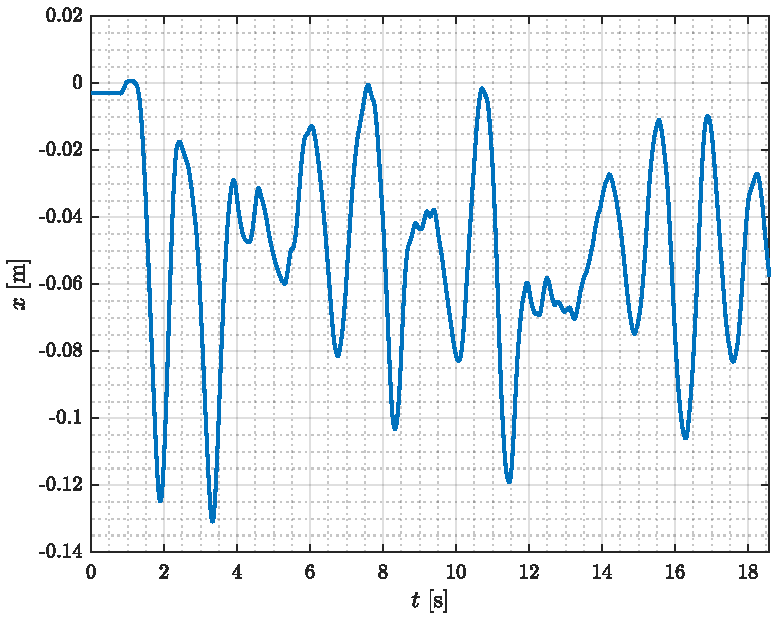
\includegraphics[width=.5\textwidth]{figures/xCatch}
  }  
\end{figure}
During test of the LQR design a problem of keeping the cart around zero on the rail was encountered. In \autoref{fig:xCatch} the controller does rather well compared to other tests. When initializing the system for each test all three encoders must be reset such that zero position is known. Originally the pendulums were reset when hanging downward and initialized to $\pi$. It was found that initializing the pendulums in upright position caused the LQR controller to converge to different parts of the rail, while with the other approach the cart consistently stayed on the right side of the rail. From this it is thought that small errors in initialized angle away from true vertical position is enough to cause an imbalance in the feedback driving the cart to one side until the position error becomes large enough to counter the angle error. On these grounds the result seen here are from a test with more fortunate initialization of the pendulum angles.\\
The control signal cooresponding to this LQR test is seen in \autoref{fig:iaCatch}.
\begin{figure}[H]
  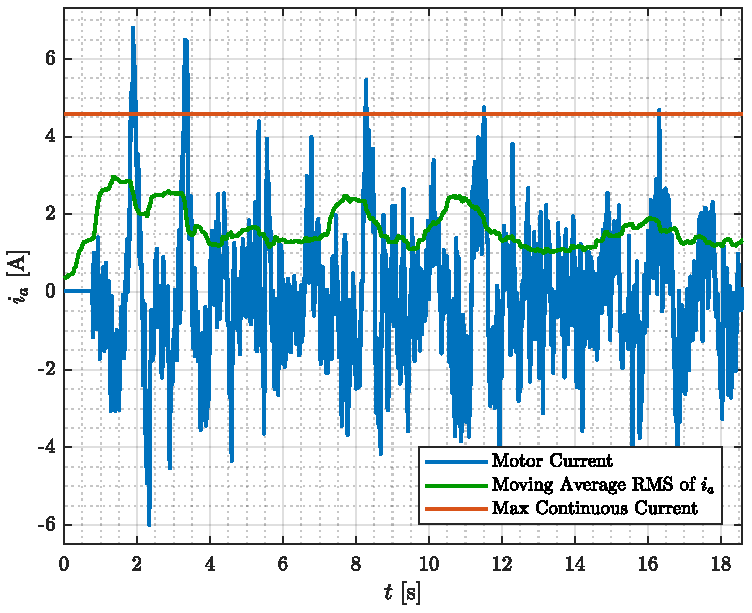
\includegraphics[width=.5\textwidth]{figures/iaCatch}
  \caption{The control signal used to achieve the results in \autoref{fig:thetaCatch} and \ref{fig:xCatch}.}
  \label{fig:iaCatch}
\end{figure}

%other available plots
% xDotCatch
% thetaDotCatch
%
%
%
In \autoref{fig:thetaSwingAttempt} the swing-up controller is tuned to $k1 = 9.5$, $k2 = 2.77$ and the energy reference of the first pendulum, $E_{\Delta_1}$, is increased by \SI{0.175}{J} while for the second pendulum $E_{\Delta_2}$ is increased by \SI{0.020}{J}. The result starts to look more like the simulations, however, in this case the first pendulum overshoots before the second pendulum reaches equilibrium. It is not known weather the LQR will be able to catch the twin pendulum even with further tuning. However, this swing-up design shows promise, that with more tuning and perhaps deploying a nonlinear control strategy for the stabilizing controller, eventually catching the twin pendulum on the given setup should be possible.
%
%------Swing-Up and Attempt Catch----------
%
%
\begin{figure}[H]
  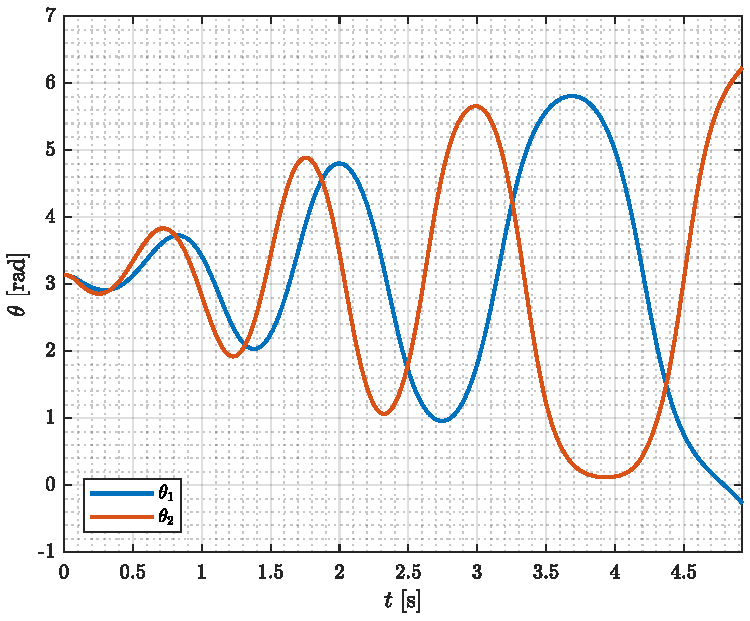
\includegraphics[width=.5\textwidth]{figures/thetaSwingAttempt}
  \caption{The swing-up controller is tuned showing promise that catching the twin pendulum on the real system should be possible with more tuning and possibly a nonlinear control strategy for the stabilizing controller.}
  \label{fig:thetaSwingAttempt}
\end{figure}
%
In the phase plot, see \autoref{fig:phaseSwingAttempt}, it is seen that the pendulums do not reach zero velocity when approaching equilibrium. The control signal used to swing up the pendulums is seen in \autoref{fig:iaSwingAttempt}, as in simulation a high but short pulse is given in the beginning of the test to start the swing-up controller.
%
\begin{figure}[H]
  \hspace{-10pt}
  \captionbox
  {
    The phase plot shows how both pendulums approach equilibrium with relatively high velocities.
    \label{fig:phaseSwingAttempt}
  }
  {
    \hspace{-1cm}
    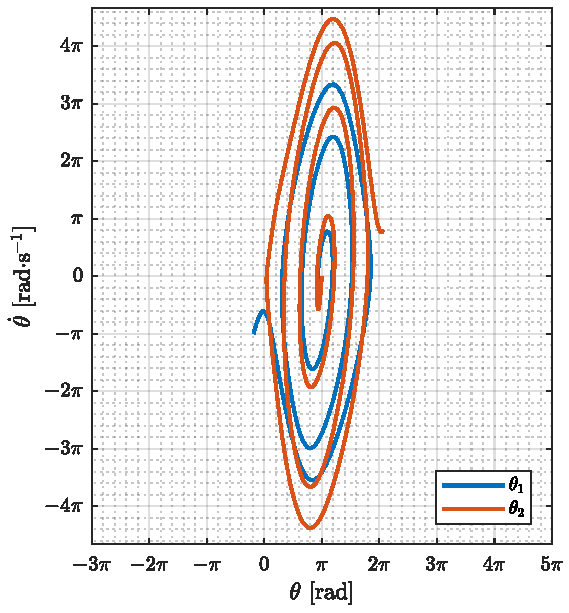
\includegraphics[width=.5\textwidth]{figures/phaseSwingAttempt}
  }
  \hspace{20pt}
  \captionbox 
  {
    The armature current is a quite high, but does not sustain high current.
    \label{fig:iaSwingAttempt}
  }
  {
    \hspace{-1cm}
    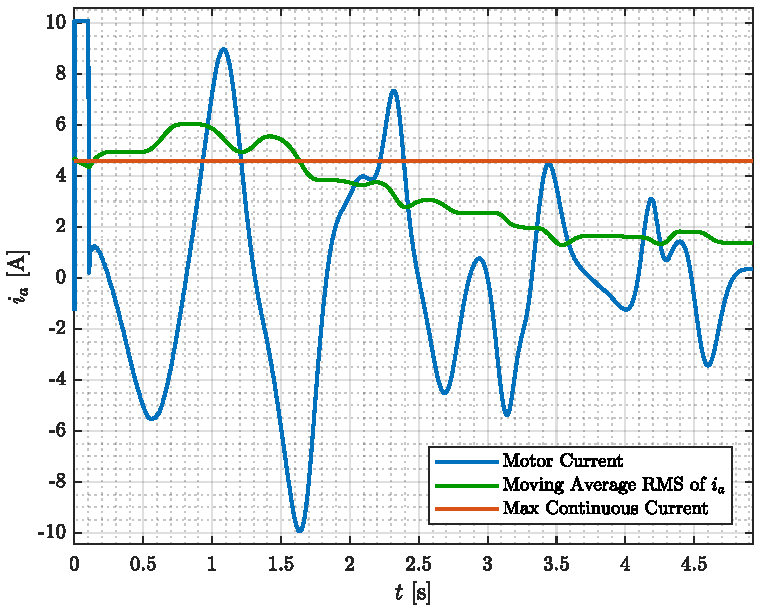
\includegraphics[width=.5\textwidth]{figures/iaSwingAttempt}
  }  
\end{figure}

%other available plots
% thetaDotSwingAttempt
% xDotSwingAttempt
% EdeltaSwingAttempt
%
The Kalman filter is implemented in c-code. The quantization problem is solved same as in simulation, see \autoref{fig:theta1KFtest} and \ref{fig:theta2KFtest} where the measurements are smoothed. The test of the Kalman filter is run with the LQR to keep the system around zero where the linear estimator is meant to operate.
%
%------Kalman Filter----------
%
\begin{figure}[H]
  \hspace{-10pt}
  \captionbox
  {
    The quantization from measurement resolution is overcome by use of the Kalman filter.
    \label{fig:theta1KFtest}
  }
  {
    \hspace{-1cm}
    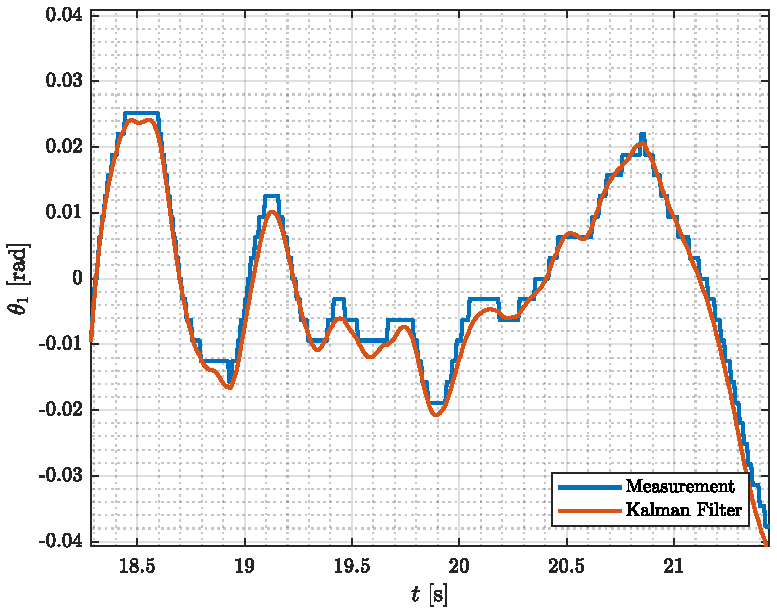
\includegraphics[width=.5\textwidth]{figures/theta1KFtest}
  }
  \hspace{20pt}
  \captionbox 
  {
    The Kalman filter shows good results for both pendulums.
    \label{fig:theta2KFtest}
  }
  {
    \hspace{-1cm}
    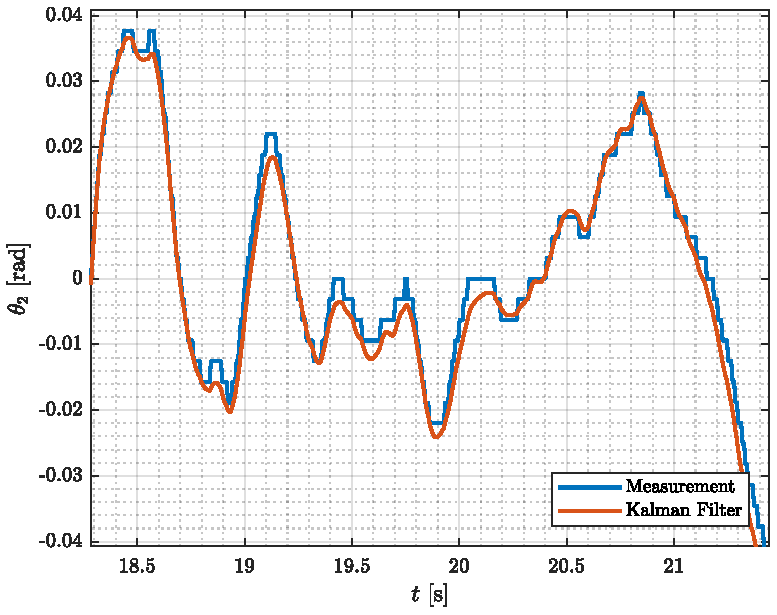
\includegraphics[width=.5\textwidth]{figures/theta2KFtest}
  }  
\end{figure}
In \autoref{fig:theta1DotKFtest} and \ref{fig:theta2DotKFtest} the Kalman filter successfully estimates the angel derivatives. An MA filter with a window size of 10 is used for comparison, notice how the MA filter is delayed compared to the Kalman filter.
\begin{figure}[H]
  \hspace{-10pt}
  \captionbox
  {
    The angular velocity of the first pendulum estimated by the Kalman filter.
    \label{fig:theta1DotKFtest}
  }
  {
    \hspace{-1cm}
    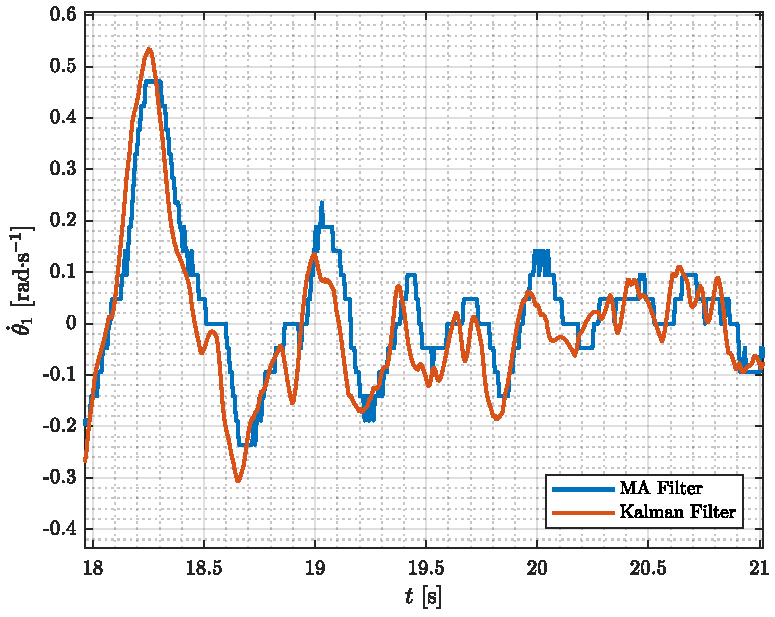
\includegraphics[width=.5\textwidth]{figures/theta1DotKFtest}
  }
  \hspace{20pt}
  \captionbox 
  {
    The velocity of the second pendulum shows similar results. 
    \label{fig:theta2DotKFtest}
  }
  {
    \hspace{-1cm}
    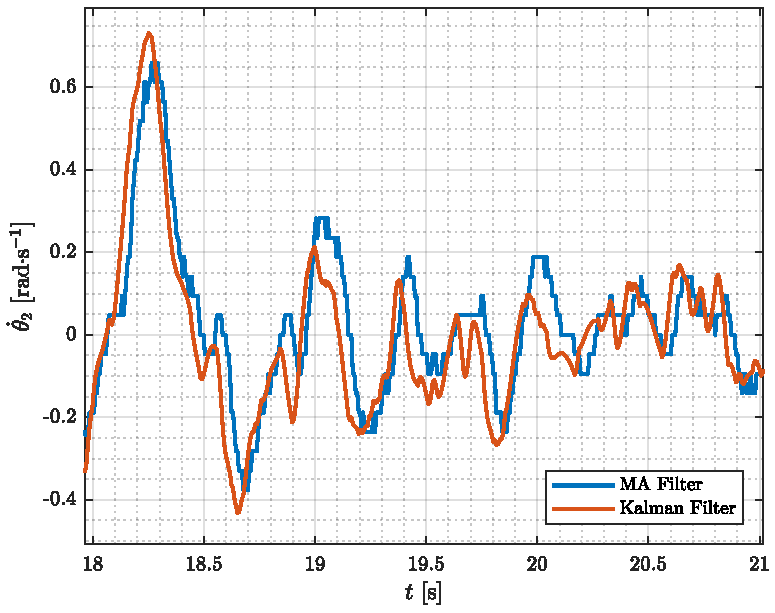
\includegraphics[width=.5\textwidth]{figures/theta2DotKFtest}
  }  
\end{figure}
%
With higher resolution on the cart position the Kalman filter shows better results and no MA filter is needed to show the trend of the derivative, see \autoref{fig:xKFtest} and \ref{fig:xDotKFtest}.
%
\begin{figure}[H]
  \hspace{-10pt}
  \captionbox
  {
    Almost no quantization noise causes no need for smoothing by the Kalman filter.
    \label{fig:xKFtest}
  }
  {
    \hspace{-1cm}
    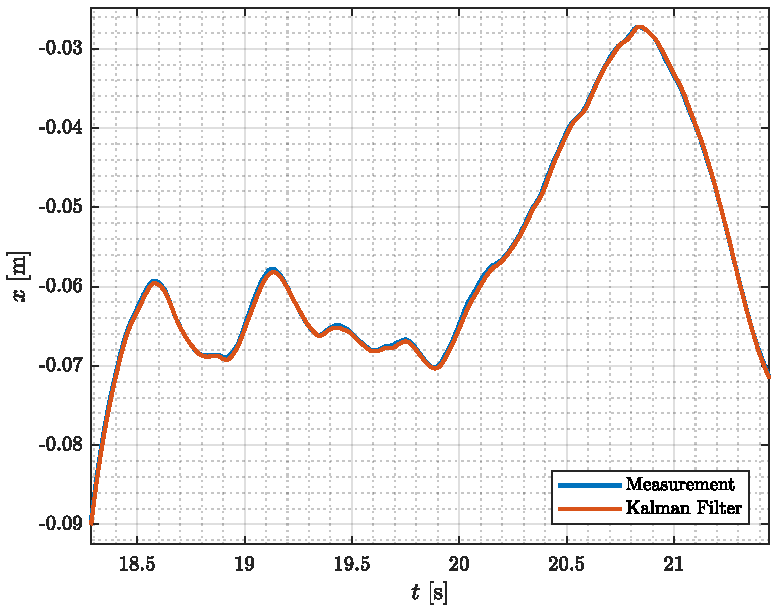
\includegraphics[width=.5\textwidth]{figures/xKFtest}
  }
  \hspace{20pt}
  \captionbox 
  {
    The estimated cart velocity leaves no noise and follows the trend of the numerical differentiation.
    \label{fig:xDotKFtest}
  }
  {
    \hspace{-1cm}
    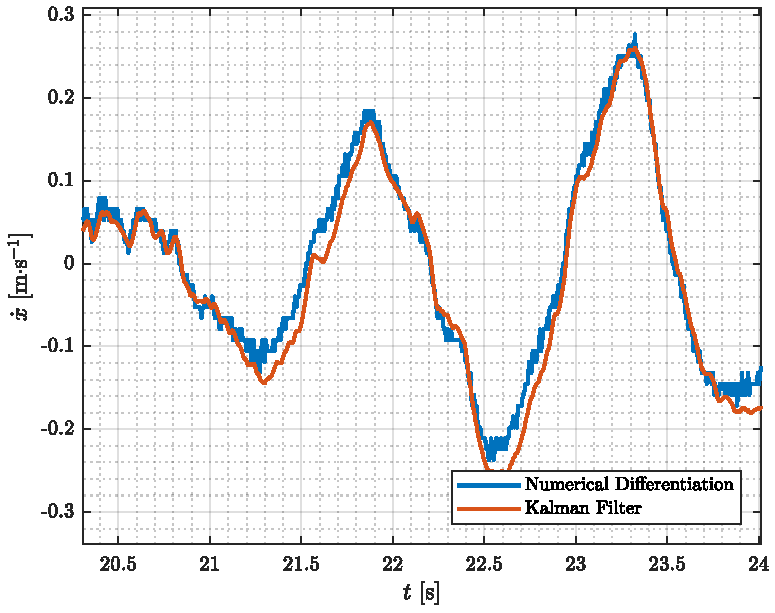
\includegraphics[width=.5\textwidth]{figures/xDotKFtest}
  }  
\end{figure}

A swing-up controller based on the principles from \textit{Part 1} was designed and successfully tested in simulation. Further, an LQR was designed to stabilize the system in zero. The stabilizing controller was in simulation capable of catching the twin pendulum after the swing-up sequence. A Kalman filter was designed and implemented to remove quantization noise form the measurements and estimate the three derivative states. Both control designs were implemented on the twin pendulum system and works separately to some degree. Catching the twin pendulum after swing-up was attempted but not successful. It is thought that further tuning of the swing-up controller and possibly a nonlinear control design for the stabilizing controller could solve this issue. This concludes \textit{Part 2} of this thesis.